\chapter{Shape Correspondence and Retrieval}
\section{Introduction}
\emph{TODO.}

\section{High Order Shape Matching}

The heat-kernel-induced signatures and distances are well suited for corresponding points on deformable shapes.
For better feature points correspondence, other than considering the similarity of point heat kernel signatures
and pair-wise heat kernel distances, we additionally take into account the compatibility of the heat kernels across
more than two points by conducting high-order graph matching on the manifold. The heat kernel tensor (HKT) is a
high-order potential of geometric compatibility of feature tuples on manifolds. To facilitate the matching process,
we further build up a two-level hierarchy via feature clustering. This simple hierarchy greatly reduces the search
space of HKT, and therefore the computation time.

Geometric relations among features are extremely important on deformable shapes, and collectively they are much
more reliable than single feature point in shape matching. Therefore, we adopt the advanced tensor
matching~\cite{Duchenne:CVPR:2011}, and transplant it to manifolds via a diffusion-driven relation measure, given by
\begin{equation}
d_{t}(x,y)=\frac{1}{4}(-t\log h_{t}(x,y))^{1/2}.
\end{equation}
Here, $h_t(x,y)$ denotes the heat kernel from point $x$ to $y$ at time $t$
\begin{equation}
h_t(x,y)=\sum_{l=0}^{\infty}e^{-\lambda_l t}\phi_l(x)\phi_l(y),
\end{equation}
where $\lambda_l$ and $\phi_l$ are the $l$-th eigenvalue and eigenfunction of the Laplace-Beltrami operator. When $t\to 0$, $d_{t}(x,y)$ is indeed a metric and converges to the geodesic between $x$ and $y$.

\begin{figure}
\centering
\includegraphics[width=0.9\linewidth]{triangle}
\caption[HKT for feature matching.]
{HKT for shape matching. Three candidate matches $(i,j,k)$ form two ``triangles''. Some outlier features are circled.}
\label{fig:triple}
\end{figure}

We consider two partial shapes $M_{1}$ and $M_{2}$ with overlaps and boundary changes. Let $N_{1}$ be the number of features extracted on $M_{1}$, and $N_{2}$ be the one on $M_{2}$. A pair $i=(i_{1},i_{2})$ denotes a candidate match with a point $i_{1}$ from $M_{1}$ and $i_{2}$ from $M_{2}$. The problem of matching point sets is equivalent to finding an assignment matrix $X_{N_{1}\times N_{2}}$, such that

\begin{equation}
\label{eq:X}
X_{i_{1},i_{2}}=
\begin{cases}
1 & \mbox{$i_{1}$ matches $i_{2}$} \\
0 & \mbox{otherwise}
\end{cases}  \mbox{, with }\sum_{i_{2}}X_{i_{1},i_{2}} \leq 1.
\end{equation}

Note that there may be outliers in the feature set. As shown in Fig.~\ref{fig:triple}, some outliers are circled. For an outlier $i_1$, there is no match in the second feature set, i.e., $\sum_{i_{2}}X_{i_{1},i_{2}}=0$. We adopt the tensor formulation~\cite{Duchenne:CVPR:2011} for high-order graph matching on manifold. Specifically, we consider a tuple of three candidate matches $(i,j,k)$ without conflicts, i.e., $i_{1}\neq j_{1}\neq k_{1}$ and $i_{2}\neq j_{2}\neq k_{2}$. They may form two ``triangles'' by connecting them with $d_t$, as shown in Fig.~\ref{fig:triple}. Since small heat kernels are error-prone, we select large heat kernels with a threshold $\epsilon_h(t)=10^{-6}$. In the case when the three points do not form a triangle, we simply drop this tuple.

The tuple of candidate matches is then embedded into a 3D space by three angles of this triangle. The distance in the embedded space is given by
\begin{equation}
d_{\theta}(i,j,k)=\|\theta_{i_{1},j_{1},k_{1}}-\theta_{i_{2},j_{2},k_{2}}\|_{2},
\end{equation}
where $\theta_{i_{1},j_{1},k_{1}}$ is a vector comprising three angles of the triangle formed by points $i_{1},j_{1},k_{1}$, and $\|.\|_{2}$ denotes the $l^{2}$-norm. The affinity of the tuple $(i,j,k)$ without conflicts is defined as

\begin{equation}
\label{eq:entry}
\tau_{i,j,k}=e^{-d_{\theta}(i,j,k)^{2}/\sigma},
\end{equation}

where $\sigma$ is a parameter, which can be set as $\sigma=\mathrm{mean} (d_{\theta})$. For tuples with conflicts, we let their affinities equal to zero. The high-order score of assignment $X$ is defined as

\begin{equation}
\mbox{score}(X)=\sum_{i,j,k} \tau_{i,j,k} X_{i_{1},i_{2}} X_{j_{1},j_{2}} X_{k_{1},k_{2}}.
\end{equation}

We rewrite the score using tensor notation, given by

\begin{equation}\label{eq:tensor}
\mbox{score}(X)=T\otimes_{1}X\otimes_{2}X\otimes_{3}X,
\end{equation}

where $\otimes_{d}$ denotes the tensor product in $d$ dimension. We call $T$ the \emph{heat kernel tensor}, as it utilizes heat kernels to form the tensor. The HKT can be fused with different order of potentials. Here, the HKT is a $3rd$-order tensor with entries $\tau_{i,j,k}$ defined in Eq.~(\ref{eq:entry}). The final results are obtained according to their matching scores subject to conflict constraints in Eq.~(\ref{eq:X}).

\begin{figure}
\centering
\includegraphics[width=0.7\linewidth]{cluster}\\
\caption[Matching hierarchy.]
{Matching hierarchy. Extracted features are clustered into sub-graphs.}
\label{fig:cluster}
\end{figure}

For articulated shapes, we design a two-level hierarchy to improve the time performance by
reducing the searching space. Articulated shapes with long branches can be easily segmented
using some low frequency eigenfunctions of the Laplace-Beltrami operator. In the upper
level, we find centers of clusters as the local extrema of the first two non-trivial
Laplace-Beltrami eigenfunctions, and remove redundant ones that are very close to selected
centers. In the lower level, extracted shape features are then clustered into sub-graphs
based on their heat kernels to the cluster centers. The goal of the upper-level matching
is to reduce the searching space, and it can be skipped whenever necessary.

The cluster centers comprise a hyper-graph in the upper level of the hierarchy, as shown in Fig.~\ref{fig:cluster}. In the hyper-graphs with hyper-nodes (cluster centers), we compute their HKT. We release conflicting constraints by allowing candidate matches that have matching scores greater than $80\%$ of the maximal one. This will prune diverse sub-graphs, and reduce the search space of HKT. At the lower level, we run HKT in each cluster. For the high-order optimization in Eq.~(\ref{eq:tensor}), we use the tensor power iteration with $l^{1}$-norms of columns. The complexity of one power iteration is $O(m)$, where $m$ is the number of non-zero elements in the tensor. We restrict the number of triangles (i.e., non-zero elements) to $64N_1$ by randomly selecting tuples. As a result, the computation of HKT is very efficient.

We conduct various experiments to demonstrate the performance, including scale change
(Fig.~\ref{fig:scale}), noise/topology change (Fig.~\ref{fig:noise})), and
large deformation  (Fig.~\ref{fig:deform}).

\begin{figure}
\centering
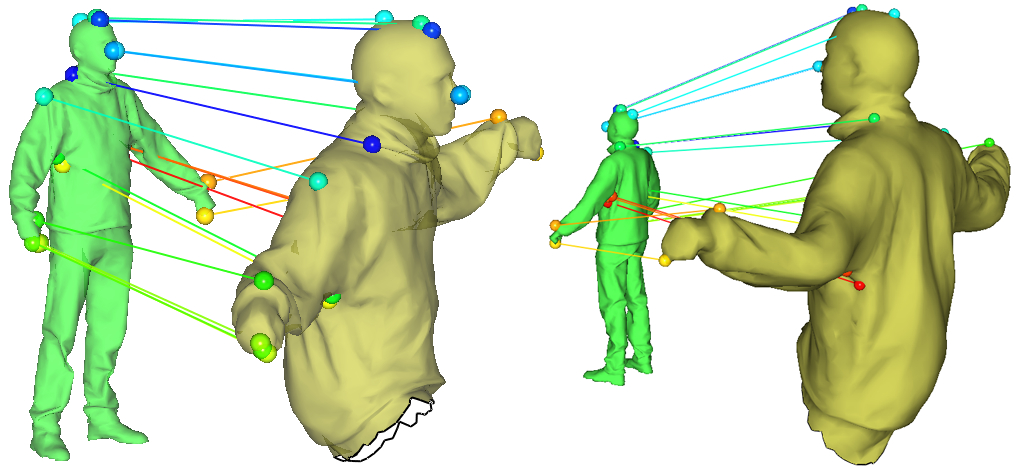
\includegraphics[width=0.9\linewidth]{scale_new}
\caption[Matching deforming shapes with scale changes.]
{Matching deforming shapes with scale changes.}
\label{fig:scale}
\end{figure}

\begin{figure}
\centering
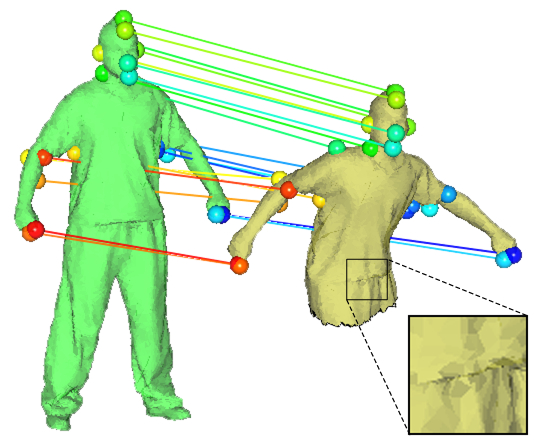
\includegraphics[width=0.45\linewidth]{noise1a}
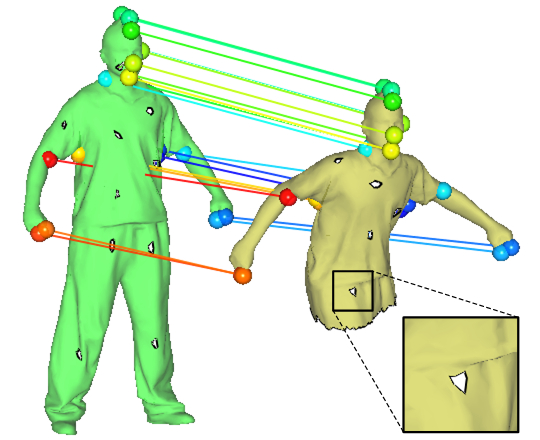
\includegraphics[width=0.45\linewidth]{noise2a}\\
\caption[Matching with noise and topology changes.]
{Matching with noise (\emph{Left}) and topology changes (\emph{Right}).}
\label{fig:noise}
\end{figure}

\begin{figure}
\centering
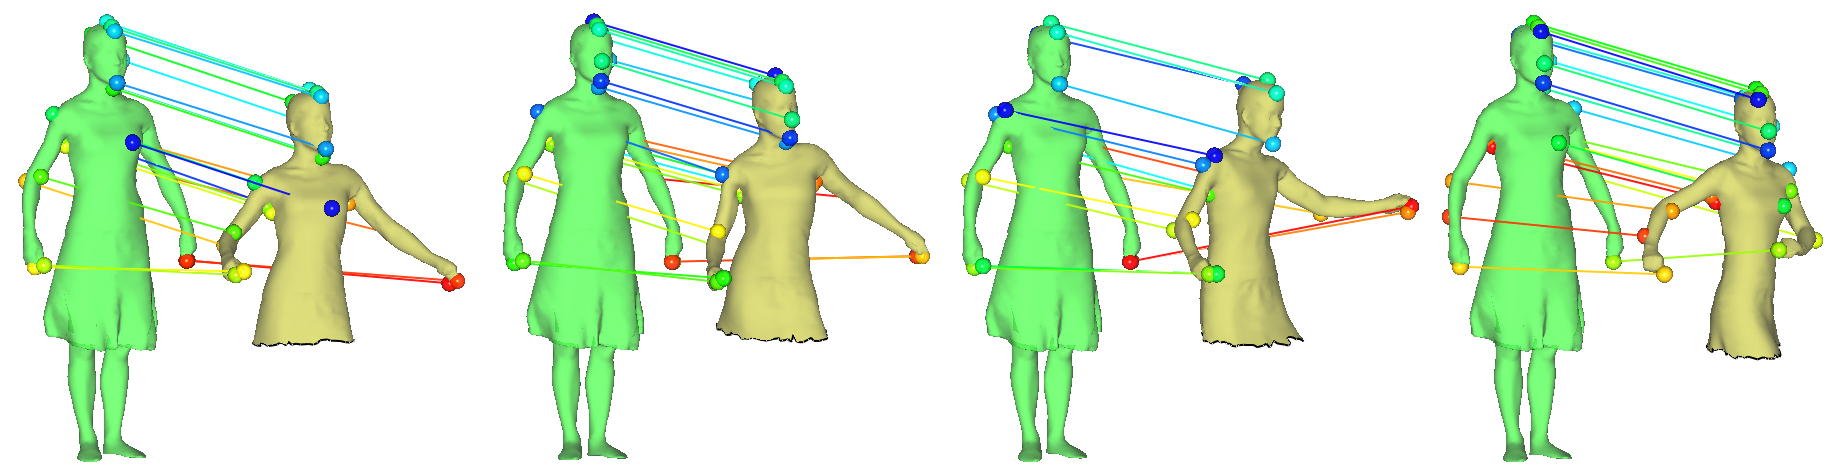
\includegraphics[width=0.9\linewidth]{deform}
\caption{Selected frames of matching objects with large deformations.}
\label{fig:deform}
\end{figure}


\section{Hierarchical Shape Registration}

We improve the registration algorithm in \cite{Hou:2011:TVCG} by implementing
a hierarchical corresponding process. The central idea is to generate correspondences
in multiple levels in a coarse-to-fine manner, with additional features incrementally
inserted in each level. The registration starts from the coarsest resolution. Registration
results obtained in one level serve as references for the registration in the next level.
We adopt the heat kernel coordinates for local shape parameterization, giving rise to a
complete solution capable of registering partial shapes undergoing isometric deformation
with higher accuracy.

A common and effective approach to dense correspondence is first matching a small number of pre-selected feature points, and then using the matched features as references for dense correspondences. Features, encoding important information of shapes, can be used to parameterize the shapes and serve as anchors to bootstrap the matching of the rest points. In general, it is necessary to have a fairly large number of matched features to obtain dense correspondence of good quality. Otherwise, the feature-based parameterization may have difficulty in discriminating nearby elements, especially in parts of shapes that are far away from any features. However, automatically finding and matching a large number of features is very difficult and error-prone. Even in the case of user-assisted feature matching, one would prefer a small set of matched features, since manually corresponding many features is burdensome and time-consuming.

\begin{figure}
\centering
  \includegraphics[width=\linewidth]{pipeline}
  \caption{Pipeline overview of our hierarchical registration framework.}
\label{fig:pipe}
\end{figure}

As illustrated in Figure \ref{fig:pipe}, the main steps of our method are: (1) Detect and match features to get a small initial set of feature matches; (2) Construct hierarchical structures of input shapes; (3) Perform registration at the coarsest level using the initial feature set; (4) Select some newly registered points as additional features; (5) Perform registration at the next level using results from the previous level and the expanded set of feature references; (6) Repeat step (4) and (5) until all valid points are registered.

The rationale of our approach is that distinguishing elements that are distant from each other on the surface is much more accurate than nearby elements. Even with a small number of features, we can achieve very good registration on a heavily downsampled version of the original shapes. The registration result of a coarse resolution can serve as seed correspondences when performing registration in a finer level. The large number of available seeds significantly reduce the chances of correspondences being trapped in an incorrect location. Moreover, the multi-resolution process enables us to pick additional features from already registered points. This greatly enhances the discriminative strength as the meshes become more refined.

%-------------------------------------------------------------------------
\begin{figure}
\centering
  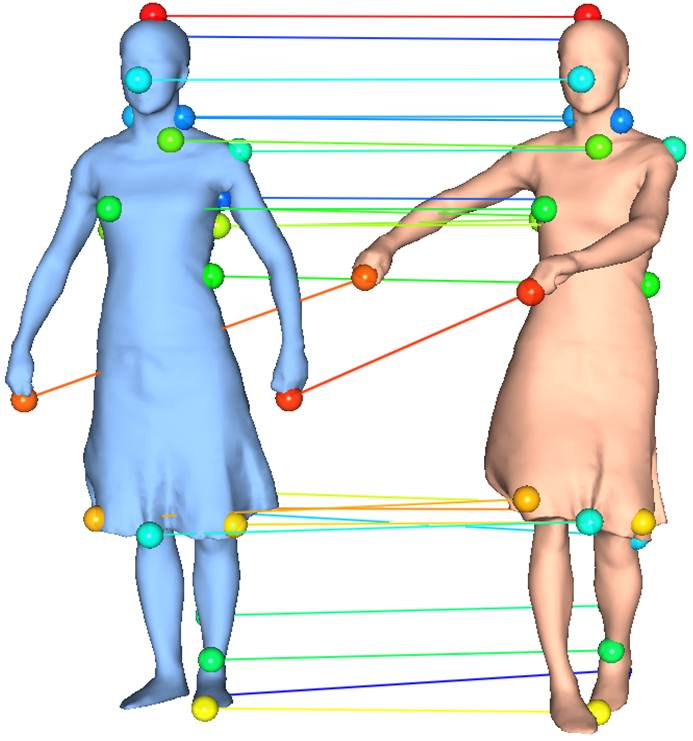
\includegraphics[width=0.2\linewidth]{comp1}
\hspace{10pt}
  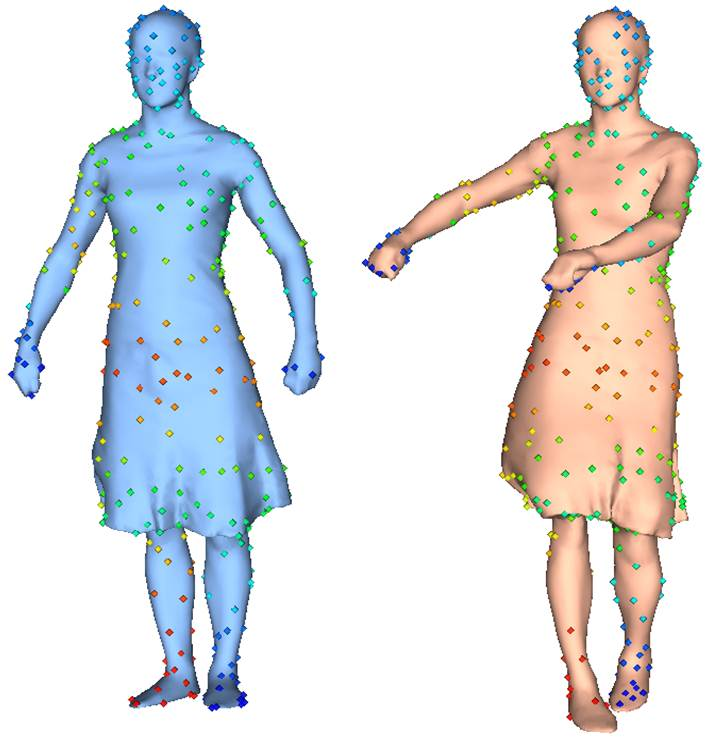
\includegraphics[width=0.2\linewidth]{comp2}
\hspace{10pt}
  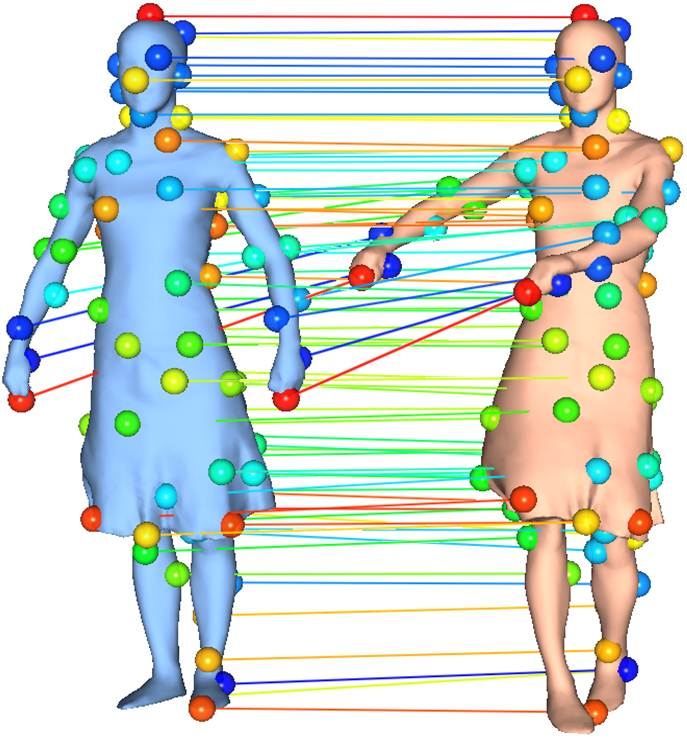
\includegraphics[width=0.2\linewidth]{comp3}
\hspace{10pt}
  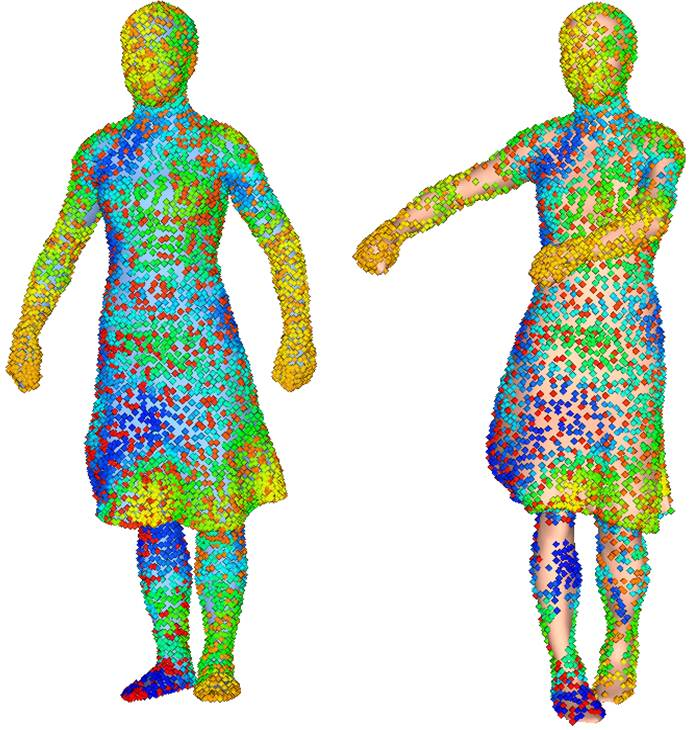
\includegraphics[width=0.2\linewidth]{comp4}\\
(a)\hspace{0.21\linewidth}(b)\hspace{0.21\linewidth}(c)\hspace{0.21\linewidth}(d)
  \caption[Steps of hierarchical registration algorithm.]
  {Major steps of our hierarchical registration algorithm. The blue shape is the source and the red one is the target. We use a three level hierarchy in this example. (a) Initial feature correspondences; (b) Coarse registration result (Third level); (c) Expanded feature correspondences (Third level); (d) Final registration result.}
\label{fig:components}
\end{figure}

\textbf{Hierarchical registration.}
Given a source shape $S$ and a target shape $T$, both represented as triangular meshes, and let $V^S=\{s_i\}$ and $V^T=\{t_i\}$ be their respective vertex sets, the objective of dense registration is to find an optimal mapping $\tau: V^S \to V^T$. In practice, we represent the registration results as a set of correspondences $R=\{v^S_i, v^T_i\}$. When the shapes in question are not complete, some vertices in $V^S$ may not have correspondences in $R$.

\textbf{Initial feature detection and matching.}
The goal of this step is to obtain a small feature correspondence set $C^*$.
In this work, we adopt the heat kernel signature (HKS) \cite{Sun:2009:CGF}
to extract multi-scale features and spectral graph matching
method \cite{Leordeanu:2005a:ICCV} to match them.

\textbf{Multiresolution Structure.}
Once we obtained features correspondence set $C^*$, we can use it as reference to propagate the correspondences by searching in the vicinity of already matched vertices, until every source vertex is mapped to a vertex in the target shape \cite{Hou:2011:TVCG,Huang:2008:CGF}. However, when the size of $C^*$ is small, simple propagation approaches often cannot produce satisfactory registration. On one hand, with insufficient features as anchors, it is difficult to distinguish nearby vertices no matter what kind of parameterization scheme we employ. On the other hand, since the sources for propagation are few, wrong correspondences are more likely to accumulate following a mismatch.

To address this issue, instead of computing registration in a single run, we perform it hierarchically in a coarse-to-fine manner. We construct a multi-resolution structure of the original shapes, and in each level we only register vertices that belong to the current resolution. Given a triangular mesh $M_0=(V_0,F_0)$ and constants $d, m \in\mathbb{Z}$, we downsample $M$ and obtain the mesh hierarchy $\{M_0,M_1,\ldots,M_m\}$. Assume $M_i=(V_i,F_i)$ and $n_i = |V_i|$, we enforce that $n_{i+1}=n_i/d$. We adopt the method in \cite{Garland:1999} for mesh downsampling. In our implementation, we select $d=4$.

\textbf{Correspondence Propagation and Feature Expansion.}
Let both the initial correspondence set $R_{m+1}$ and initial feature set $C_{m+1}$ be $C^*$. In level $l$, we input the previous level's registration result $R_{l+1}$ and feature set $C_{l+1}$. The goal is to find the $l$-th level correspondence set $R_l$ that registers meshes $S_l$ and $T_l$, with an augmented feature set $C_l$.

For each vertex $x$ in $S_l$ and $T_l$, we compute its heat kernel coordinates
\begin{equation}
\HKC(x)=(h_t(x,c_1),\dots,h_t(x,c_z)) \mbox{, } c_i\in C_{l+1}.
\end{equation}

Inheriting $R_{l+1}$ as the initial correspondence set, we propagate correspondence to match the rest vertices in $S_l$ and $T_l$. We use a heap to determine the order by which the vertices in $S_l$ are processed, prioritizing on the magnitude of HKC. For an already matched pair $(s_j, t_j)$ and one of $s_j$'s immediate neighbor $s_i$, we search for $s_i$'s best correspondence $t_i \in V^T_k$ in the neighborhood of $t_j$, and add $(s_i,t_i)$ into the correspondence set. $t_i$ is selected using the following criterion
\begin{equation}
t_i=\argmin_{t\in n(t_j,T_k)}\|{\HKC}_S(s_i)-{\HKC}_T(t)\|_2
\end{equation}
where $n(t_j,T_k)$ represent the set of $t_j$'s neighboring vertices in $T_k$, and $\HKC_S$ and $\HKC_T$ denote the heat kernel coordinates of points on $S$ and $T$.

The correspondence propagation continues until all vertices in $S_k$ have been matched and we get the correspondence set $\{(s_i,t_i)\} \subset V^S_{m-1} \times V^T_{m-1}$. Note that for each correspondence $(s_i,t_i)$, the endpoint $t_i$ actually represent a set of vertices $K(t_i)$ in the original mesh $T_0$. To find the precise correspondence of $s_i$ in the original target mesh, we search $K(t_i)$ and replace $t_i$ with $t_j \in K(t_i)$ if $t_j$ is closer to $s_i$ in the embedding space. The result is the $l$-th level correspondence set $R_k$ that relates points $s_i \in S_k$ to $t_i \in T_0$. For each correspondence $(s_i,t_j)$, we assign a matching score
\begin{equation}
score(s_i,t_j)=\exp(-\|{\HKC}_S(s_i)-{\HKC}_T(t_j)\|_2).
\end{equation}

We then select from $R_l$ some vertex pairs as new features and insert them into the feature set. These new added feature pairs should be both reliable (having great matching score) and not in the $\delta$-neighborhood of any existing feature points. The expanded feature set $C_l$ enables a more discriminative HKC in the next level. We carry on this process from the coarsest level to the finest level until we obtain the final registration set $R_0$ between the original meshes $S_0$ and $T_0$.
Fig.~\ref{fig:components} shows the major steps of our algorithm.

\begin{figure}\centering
  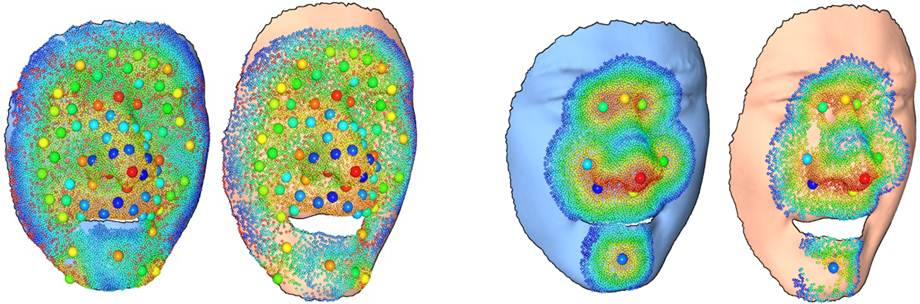
\includegraphics[width=0.45\linewidth]{face_cmp}
  ~
  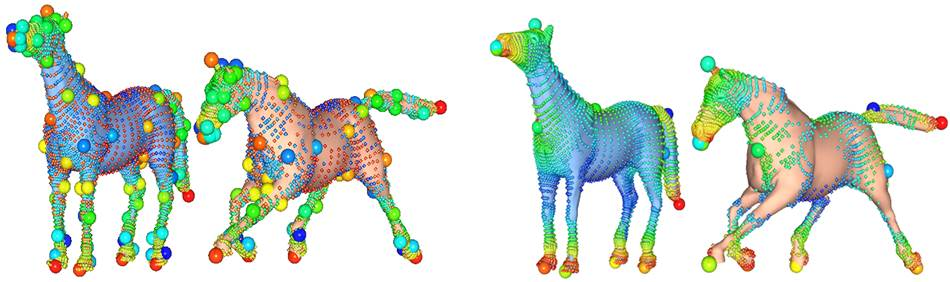
\includegraphics[width=0.45\linewidth]{horse_cmp}
  \\
  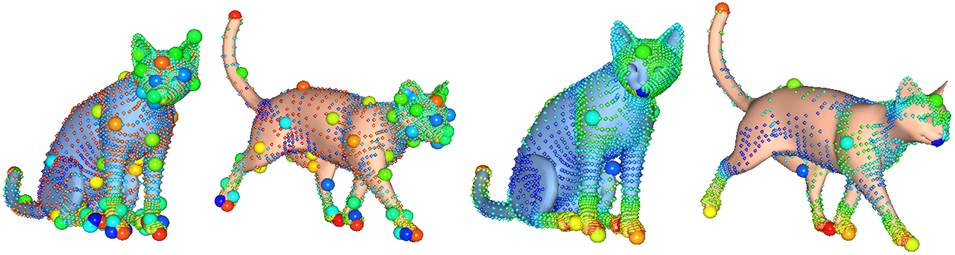
\includegraphics[width=0.45\linewidth]{cat_cmp}
  ~
  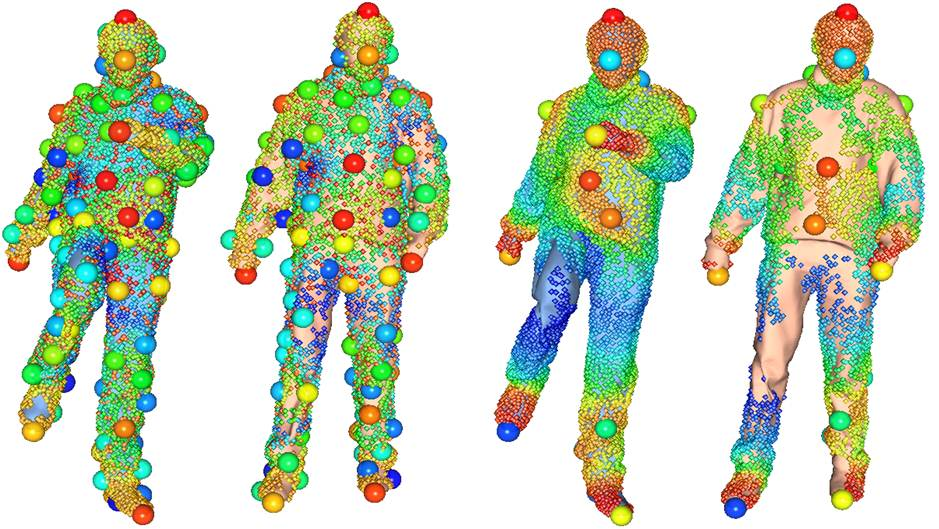
\includegraphics[width=0.45\linewidth]{man_cmp}
\caption[Registration results using multi-resolution method.]
 {Some registration results using our multi-resolution method (\emph{Left}) and the single-resolution method \cite{Hou:2011:TVCG} (\emph{Right}). Large colored dots represent matched features.}
\label{fig:results}
\end{figure}

\section{Bag-of-Feature-Graphs Shape Retrieval}

In Chapter~5, we have articulated an informative shape region descriptor which incorporates spectral graph wavelet coefficients
and contour-related statistics for improved discriminative power. This new descriptor is robust and near-isometry-invariant, and
we have demonstrated its great performance in matching and retrieving interesting shape regions.

We plan to employ our regional feature descriptor for whole shape retrieval from a database. Existing shape retrieval
methods usually rely on the aggregation of local point features, such as shape context~\cite{Belongie2002} and
heat kernel signature~\cite{Sun:2009:CGF}. Comparing with point features, our region features can better describe
the contour shape and local-global geometry of interesting shape regions. In addition, the detected feature regions
are much more intuitive for interpretation than point features.

The general pipeline for feature-based shape retrieval is as follows:
\begin{enumerate}
\item Detect regional shape features from a training set of shapes. Each detected region is represented using our region descriptor.
\item Learn a set of representative vector in the region descriptor space through clustering, forming a vocabulary of ``geometric words''.
\item For each query or target shape, encoding its detected regional features against the vocabulary via some local feature aggregation method
on manifold.
\item Compute shape similarities by comparing the shape descriptions obtained in the above step.
\end{enumerate}

To effectively characterize a shape, only using the distribution of word frequency as in
traditional bag-of-words method is not enough. We need to incorporate the spatial relations
between features into our representation, and the most effective way to encode pairwise
relation is through graph-based feature aggregation method, such as spatially sensitive
bags of features (SS-BoF)~\cite{Bronstein2011}, bags of feature graphs (BoFG)~\cite{Hou2012a},
and relevance diffusion~\cite{Furuya2015}.

We present a new paradigm, called bag-of-feature-graphs (BoFG), for non-rigid shape retrieval. The basic idea is to represent a shape by constructing graphs among its features, which significantly reduces the number of points involved in computation. Given a vocabulary of geometric words, for each word the BoFG builds a graph that records spatial information of features, weighted by their similarities to this word. This eliminates unlikely points in a word category, during shape comparison. Feature graphs are governed by their affinity matrices of weighted heat kernels, whose eigenvalues form a concise shape descriptor. Given a vocabulary of geometric words, corresponding to each word we build a graph that records spatial information between features, weighted by their similarities to this word. Specific characteristics of the BoFG include:
\begin{itemize}
\item It is concise by significantly reducing the number of points involved in representation, and thus, is fast to compute.
\item It explicitly records spatial information among features.
\item It is representative, since features are salient points
containing important information of the shape.
\item Graphs have different dominating features associated with corresponding words. This greatly improves the accuracy of shape comparison by eliminating unlikely word-distributions.
\end{itemize}

\begin{figure}
\centering
\includegraphics[width=0.9\linewidth]{bowm}\\
BoW vector ($V \times 1$)\\
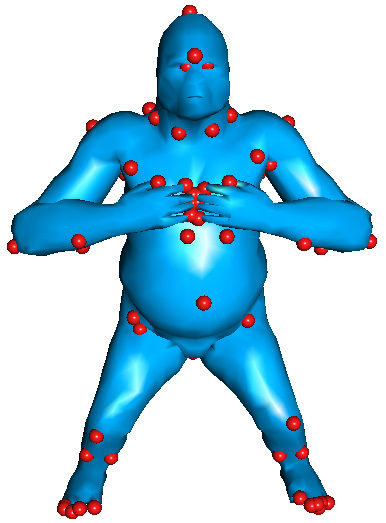
\includegraphics[width=0.35\linewidth]{gorilla}
\hspace{20pt}
\includegraphics[width=0.38\linewidth]{ssbowm}\\
\hspace{30pt} Shape \hspace{46pt} SS-BoW matrix ($V \times V$)\\
\includegraphics[width=0.3\linewidth]{bofgm_1}
\includegraphics[width=0.3\linewidth]{bofgm_2}
\includegraphics[width=0.3\linewidth]{bofgm_3}
\dots\\
BoFG matrices ($|F| \times |F| \times V$)
\caption{Different representations of a given shape.}
\label{fig:represent}
\end{figure}

We first revisit the `Shape Google' method originally introduced in \cite{Ovsjanikov:2009}. It utilizes a HKS-based BoW.
The HKS descriptor $K(x)$ is a vector of HKS sampled at different values of $t$. Let $\textbf{W}=\{W_1,\dots,W_V\}$ be a
vocabulary of geometric words with size $V$. The words $\{W_i\}$ are representative HKS vectors in the descriptor space
clustered by the k-means algorithm. For each point $x$, the shape google computes its word distribution
$\Theta(x)=[\theta_1(x),\dots,\theta_V(x)]^T$. The similarity of $x$ and word $W_i$ is given by

\begin{equation}\label{eq:similar}
\theta_i(x)=c(x)e^{-\frac{\|K(x)-W_i\|^2}{2\sigma^2}},
\end{equation}

where $\sigma$ is a parameter, and $c(x)$ is the normalization factor selected such that $\|\theta(x)\|_1 = 1$.
The BoW descriptor of a surface $M$ is computed by integrating word similarities over the entire shape

\begin{equation}
f(M)=\int_M\Theta(x)d\mu(x),
\end{equation}

where $\mu(x)$ denotes the surface area of $x$. As shown in Fig.~\ref{fig:represent},
the BoW descriptor is a V$\times$1 vector that measures the frequencies of words appearing
on the shape. The shape google also introduced a SS-BoW descriptor, given by

\begin{equation}
F(M)=\int_{M\times M}\Theta(x)\Theta^T(y)h_t(x,y)d\mu(x)d\mu(y).
\end{equation}

As shown in Fig.~\ref{fig:represent}, it is a V$\times$V matrix that measures frequencies of word pairs. Assume the time complexity for computing a HKS descriptor is O(D). For a shape with N points, the time complexity of BoW is O(ND), and SS-BoW is O($N^2 D$) which is quadratic to N.

According to the Informative Theorem in \cite{Sun:2009:CGF}, the HKS contains all the information of heat kernels. Thus, the SS-BoW has no more geometry information than the BoW before integration. For the ease of comparison, the shape google highly suppresses the geometry information by computing the frequencies of words or word-pairs on the shape. It ends up with concise descriptors for comparison, yet completely loses spatial information. Besides, the shape-google algorithms are time-consuming, since they are working on all the points in the data. The BoW needs computing HKS values of all points, while the SS-BoW needs computing all point-to-point heat kernels. Assume the time complexity for computing a HKS descriptor is O(D). For a shape with N points, the time complexity of BoW is O(ND), and SS-BoW is O($N^2 D$) which is quadratic to N.

To reduce the complexity of the shape google, one needs to reduce the number of points involved in representing the shape. A straightforward solution is to select feature points, which keep most information of the shape geometry. Because of the multi-scale property, HKS features contain geometry information ranging from points in small scales to the entire shape in large scales. However, one concern is that a reduced number of points may not be sufficient to faithfully represent the shape. Therefore, instead of counting word frequencies, we construct graphs on detected features, giving rise to a bag-of-feature-graphs (BoFG) paradigm. The graphs encode spatial relations between features, which contain much more geometry information in representing the shape.

We adopt weighted heat kernel matrices to capture global structures of graphs. Specifically, for a shape $M$ with feature set $F$, only points $x\in F$ are involved in computing word distributions $\Theta(x)$, which reduces much computation. Features are vector-quantized by a fuzzy classification, which assigns $\theta_i(x)$ portion of similarity to word $W_i$ in the distribution of feature $x$. The distribution $\Theta(x)$ is computed by Eq.~(\ref{eq:similar}) with $\sigma$ set as $\frac{1}{4}$ of the average distance of words in the vocabulary. This fuzzy classification reduces ambiguities in graph comparison, and also avoids misclassification in a hard quantization. For a geometric word $W_i$, we construct a matrix $G_i$, whose entry $G_i(x,y)$ with $(x,y)\in F\times F$ is computed by,
\begin{equation}
G_i(x,y)=\theta_i(x)\theta_i(y)h_t(x,y).
\end{equation}
It is the heat kernel between $x$ and $y$ weighted by their similarities to the geometric word $W_i$.

The matrix set $\textbf{G}(M)=\{G_1,\dots,G_V\}$ comprises a BoFG representation of the shape $M$. As shown in the bottom row of Fig.~\ref{fig:represent}, matrices characterize spatial information of features assigned to different word categories. The near-zero entries in a matrix indicate they are hardly classified to this category, and therefore, not considered in this graph. It contains all the geometric information of features in a multi-scale way, which faithfully characterizes the shape. The computation complexity for this matrix representation is O($|$F$|^2$D), as the computed heat kernels can be shared by all matrices. Considering the size of feature set is always much less than the total number of points on the shape, the BoFG is much faster than the shape google.

\begin{figure}
\centering
\includegraphics[width=0.9\linewidth]{eigen}
\caption[Nonrigid shapes and their BoFG descriptors.]
{Some non-rigid shapes and their BoFG descriptors.}
\label{fig:eigen}
\end{figure}

The mechanism of shape retrieval is to build concise BoFG descriptors of shape models in a database in an off-line process, and retrieve related shapes for a query by the approximate nearest neighbor (ANN) search. The BoFG descriptor consists of significant eigenvalues of BoFG matrices. Each $G_i$ is a real symmetric matrix, whose eigenvalues are all real and eigenvectors are perpendicular to each other. We choose its six largest eigenvalues denoted as $S_i(M)$, which contributes to a 6V$\times$1 vector $[S_1(M),\dots,S_V(M)]^T$ as a concise descriptor. This reduces the dimension of the matrix by multi-dimensional scaling (MDS) \cite{Bronstein2006}. Fig.~\ref{fig:eigen} shows some non-rigid shapes and their BoFG descriptors. The deformed cat-models have very similar BoFG descriptors, while the horse-model has a quite different one. It projects the matrix to its main directions with coordinates leaving in $S_i(M)$, which are stable to a small amount of outliers. Then, we define the similarity distance between two shapes $M_1$ and $M_2$ as
\begin{equation}
d(M_1,M_2)=\sum_{i=1}^{V}\|S_i(M_1)-S_i(M_2) \|_2.
\end{equation}

The above distance is based on one-scale heat kernels, which can be easily extended to multi-scale by averaging distances of heat kernels at different values of $t$.

\section{Chapter Summary}
\emph{TODO.} 